%   File: CrossProduct.tex
% Author: Adam Leeper
%------------------------------------------------------------------------------
%\\[0.45pc]
\providecommand{\isolatedBuild}[1]{#1}% fallback definition lets this file build normally
\isolatedBuild{
  \documentclass[11pt,letterpaper]{article}
  %\documentclass[11pt,letterpaper]{book}

% aleeper: I think these are needed for Paul's macros?
\usepackage{epsfig}
\usepackage{epstopdf}

%\makeatletter
%\typeout{The import path is \import@path}
%\makeatother

\usepackage{import}

\subimport{./}{packagesMitiguy.sty}
\subimport{./}{macrosMitiguy.tex}
\subimport{./}{PageStylesMitiguy.tex}
\subimport{./}{macrosLeeper.tex}
 % Requires the TEXINPUTS environment variable.
  \isolatedBuildHeader
    {Rotational Kinematics}
    {Dynamics of a Rider on a Ferris Wheel}
  %\vspace{-2.0pc}
  \\[0.0pc]
}
%%%
%%%
%%%
\begin{minipage}{1.0\linewidth}
  \begin{minipage}[t]{0.60\linewidth}
    The figure at right shows a Ferris wheel.
    We take the ground to be a Newtonian reference frame \basis{N}.
    \Dextral, orthogonal unit-vectors \uvecxyz{n} are fixed in \basis{N}
    as shown (\uvecx{n} is out of the page).
    %
    \\[0.5pc]
    The Ferris wheel \basis{B} spins \textbf{counter-clockwise} at a
    variable rate $\omega$ and has chairs located at a radius $R$ from the
    center point $B_o$.
    The rider sits on (and is fully supported by) a bathroom scale.
    We simplify the problem by modeling the rider as a particle $Q$ and
    assuming that the seat is always exactly horizontal.
    %
    \\[0.5pc]
    \textbf{Hint:} The concept of a rigid frame \basis{B} is needed,
    but unit vectors fixed on \basis{B} are \textbf{not} needed.
    Instead, use formulas for two points fixed on a rigid body.
  \end{minipage}
  \hfill
  \begin{minipage}[t]{0.35\linewidth}
    \vspace*{-5pt}
    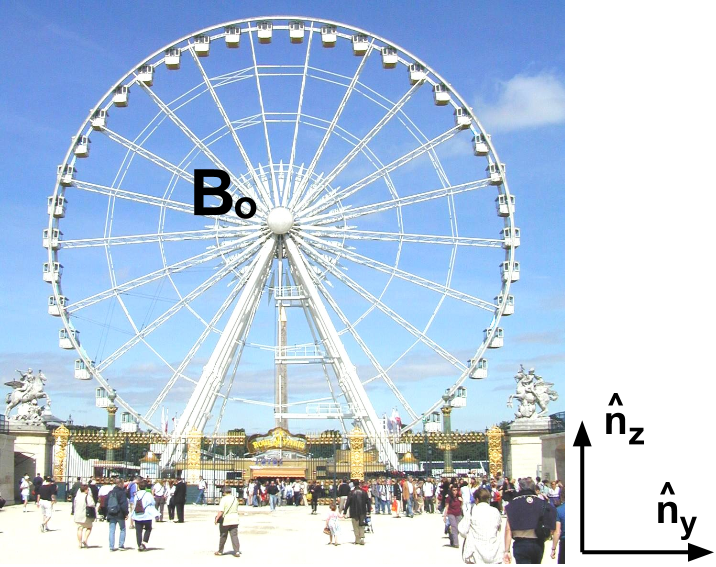
\includegraphics[width=1.0\linewidth]{ferris_wheel.png}
  \end{minipage}
\end{minipage}
%
\\[0.0pc]
\begin{enumerate}
  \item Write down the angular velocity and angular acceleration
        of \basis{B} in \basis{N}.
        %
        \\[0.45pc]
        $\angvel{B}{N}\equals[\;] \hidemath[0.7cm]{ \omega ~\uvecx{n} }$
        \hspace{3cm}
        $\alf{B}{N}\equals[\;] \hidemath[0.7cm]{ \dot{\omega} ~\uvecx{n} }$
        \\[0.45pc]
        \Solution {}{1.0\linewidth}{
          The Ferris wheel is undergoing ``simple'' rotation
          (see section 7.3.3), so angular velocity is formed
          \textbf{by inspection}.
          The rotation rate is given above as the variable $\omega$,
          and the direction is picked by curling the fingers of your
          right hand to follow the counter-clockwise rotation, resulting in
          your thumb pointing out of the page in the $+\uvecx{n}$ direction.
          \\[0.45pc]
          For angular acceleration we use the definition,
          $\alf{B}{N} \deff[\;] \dt[N]{}\angvel{B}{N}$, which is
          straight-forward since \uvecx{n} is fixed in \basis{N}.
        }
        \\[0.0pc]
        %
  \item Find an expression for the rider's acceleration in \basis{N}
        \boldUnderlineDarkRed{at the instant} when he is at the
        \boldUnderlineDarkRed{top} of the
        Ferris wheel, in terms of previously defined symbols and \uvecxyz{n}.
        %\\[0.0pc]
        \textbf{Hint:} What is $\posvec{B_o}{Q}$ at that instant?
        \\[0.5pc]
        $\accel{Q}{N} \equals[\;] \hidemath[0.7cm]{ \minus[\;]
        \dot{\omega} R ~\uvecy{n} \minus[\;] \omega^2 R ~\uvecz{n}}$
        \\[0.45pc]
        \Solution {}{1.0\linewidth}{
          Point \origin{B} is fixed in \basis{N}, so we might be
          tempted to form the position vector,
          $\posvec{\origin{B}}{Q} \equals[\;] R~\uvecz{n}$,
          and differentiate.
          However, this vector is only valid at the
          \boldUnderlineDarkRed{instant} $Q$ is at the top of the wheel
          (a short time before or after this instant, the direction from
          \origin{B} to $Q$ would include some \uvecy{n} component), so
          it is \boldUnderlineDarkRed{invalid} to differentiate it.
          (As we have done in other problems, one approach would be to
          introduce a basis fixed on \basis{B} so that
          $\posvec{\origin{B}}{Q}$ could be written in a form that is
          valid for all time.)
          %
          \\[0.45pc]
          Instead, since \origin{B} and $Q$ are both fixed on \basis{B},
          the equations for velocity and acceleration of two points fixed
          on a rigid body apply (Mitiguy section 8.2).
          \\[0.45pc]
          \begin{tabular}{l@{\equals[\;]}c@{}c@{}c@{}c@{}cl}
              $\accel{Q}{N}$
              & $\accel{\origin{B}}{N}$
              & $\plus[\;]$
              & $\alf{B}{N} \CrossProduct \posvec{\origin{B}}{Q}$
              & $\plus[\;]$
              & $\angvel{B}{N} \CrossProduct
                  (\angvel{B}{N} \CrossProduct \posvec{\origin{B}}{Q})$
              & General equation valid for all time.
            \\[0.2pc]
              & $\zerovec$
              & $\plus[\;]$
              & $\omegadot~\uvecx{n} \CrossProduct R~\uvecz{n}$
              & $\plus[\;]$
              & $\omega~\uvecx{n} \CrossProduct
                  (\omega~\uvecx{n} \CrossProduct R~\uvecz{n})$
              & Valid at this instant due to expression for
                \posvec{\origin{B}}{Q}.
            \\[0.2pc]
              & $\zerovec$
              & $\plus[\;]$
              & $\omegadot~R~(-\uvecy{n})$
              & $\plus[\;]$
              & $\omega~\uvecx{n} \CrossProduct
                  (\omega~R (-\uvecy{n}))$
              &
            \\[0.2pc]
              & $\zerovec$
              & $\plus[\;]$
              & $\omegadot~R~(-\uvecy{n})$
              & $\plus[\;]$
              & $\omega^2~R~(-\uvecz{n})$
              &
          \end{tabular}
          \\[1.0pc]
        }
        \\[0.0pc]
        %
  \item The forces on the rider might be modeled as: a horizontal
        friction force $F_y$ and vertical support
        force $F_z$ from the scale; and gravity.
        Hence, $\force{Q} = F_y~\uvecy{n} + (F_z - m^Q g) ~\uvecz{n}$.
        Plug $\force{Q}$ and your result for
        \accel{Q}{N} into Newton's law to get a vector equation, then dot
        with a unit vector to get a scalar equation relating $F_z$
        and $\omega$.
        \\[0.45pc]
        \Solution {}{1.0\linewidth}{
          \begin{tabular}{r@{~\equals[\;]~}ll}
              $\force{Q}$
              & $\mass{Q} \mult[\;] \accel{Q}{N}$
              &
            \\[0.2pc]
                $F_y~\uvecy{n} + (F_z - m^Q g) ~\uvecz{n}$
              & $\mass{Q} \mult[\;] (\minus[\;] \omegadot R ~\uvecy{n}
                                     \minus[\;] \omega^2 R ~\uvecz{n})$
              & $F_z$ is in an \uvecz{n} term, so we'll dot with \uvecz{n}.
            \\[0.2pc]
                $F_z - m^Q g$
                & $\minus[\;] \mass{Q} \mult[\;] \omega^2 R$
              & This could be solved for any scalar of interest.
          \end{tabular}
          \\[1.0pc]
        }
        %\\[0.0pc]
        %
%  \item The wheel has radius $R = 10$ meters and the rider has mass
%        $m^Q = 80$ kg. However, at the \textbf{top} of the Ferris wheel
%        the bathroom scale reads $F_z = 700$ Newtons.
%        Assume $g = 10\frac{\mathrm{m}}{\mathrm{sec}^2}$ for simplicity.
%        Determine the rotation rate $\omega$ of the wheel at that instant.
%        \\[1.0pc]
%        $\omega \equals[\;] \hidemath[1cm]{\sqrt{\frac{m^q g - F_y}{m R}}}$
%        \\[25.0pc]
%        \vfill
%
%  \item Find an expression for the velocity in \basis{N} of the rider
%        \textbf{at the instant} he is at the \textbf{top} of the Ferris
%        wheel, in terms of previously defined symbols and \uvecxyz{n}.
%        \\[0.5pc]
%        $\vel{Q}{N} \equals[\;]
%         \hidemath[0.7cm]{ \minus[\;] \omega R ~\uvecy{n} }$
%        \\[10.0pc]
%
%  \item If you differentiate in \basis{N} your result from (e), you
%        \choiceAB{DO}{DO NOT}{1} get the same expression as in (b).
%        Explain why.
%        \\[8.0pc]
\end{enumerate}
%
\isolatedBuildFooter
